\section{Introduction}\label{sec:intro}


As Artificial General Intelligence (AGI) has developed rapidly, it has led to influential applications such as ChatGPT in Natural Language Processing (NLP) and Midjourney in Computer Vision (CV). However, work on graph data is still at an early stage compared with the progress achieved in NLP \cite{
devlin2019bert,
brown2020language, liu2023pretrain} and CV areas \cite{
% radford2021learning,
% li2022blip,
% zhu2023minigpt4,
wang2023chatvideo,
zhang2023videollama}. In an increasingly interconnected world, graphs are important for modeling relational data and extracting useful patterns. This has drawn growing academic and industrial interest in AGI for graph data \cite{liu2023graph, zhang2023large, yang2023datacentric}, with promising applications in areas such as drug design \cite{rong2020selfsupervised, qian2023can} and battery development \cite{wang2023scientific}.




\begin{figure}[!t]
    \centering
    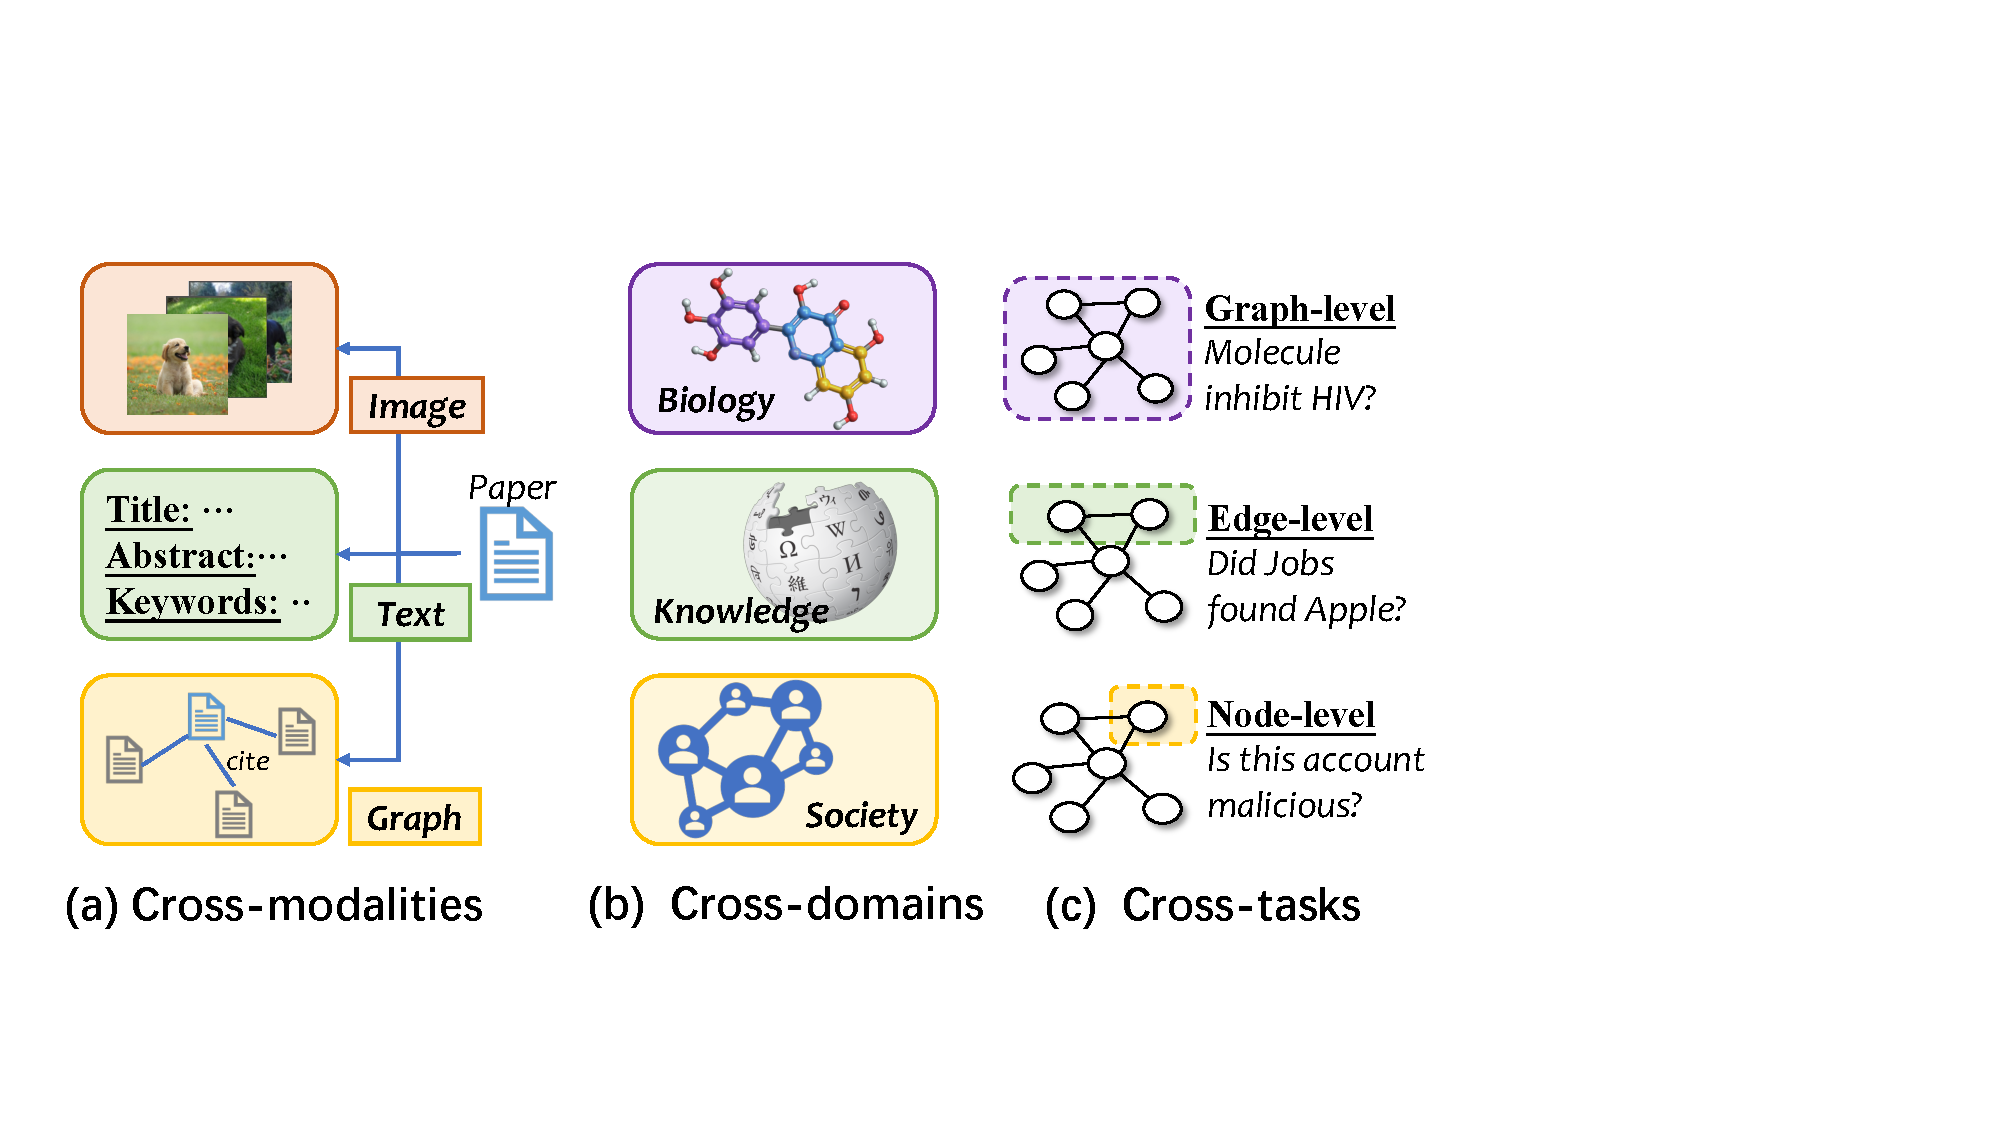
\includegraphics[width=0.45\textwidth]{pic/ThreeChallenges}
    \caption{The Most Frequent Problems towards Artificial General Intelligence. (a) Cross-modalities, (b) Cross-domains, (c) Cross-tasks.}
    \label{fig:AGIProblems}
\end{figure}



However, realizing this vision is difficult. Figure \ref{fig:AGIProblems} illustrates this landscape in recent AGI research and highlights at least three fundamental technical challenges: \textbf{\textit{(1) How to make the model general for different modalities?}} Within the NLP and CV areas, there have been many commercial models that can understand and translate information across these modalities \cite{
devlin2019bert,
% radford2021learning,
% li2022blip,
% zhu2023minigpt4,
zhang2023videollama,
brown2020language}. For example, models like BERT \cite{devlin2019bert} and GPT-3 \cite{brown2020language} have demonstrated the ability to perform tasks that involve both textual and visual information. However, in the context of graph data, integrating information from multiple modalities remains largely uncharted territory \cite{li2023graphadapter}.
% he2023explanations,
% yoon2023multimodal,
% li2023graphadapter
% chen2023exploring
\textbf{\textit{(2) How to make the model general for different domains?}} For the cross-domain issue, transfer learning has proven effective, enabling models to apply knowledge learned from images and text in one domain to another. However, transferring knowledge between different graph domains is difficult because the semantic spaces are not aligned \cite{zhu2023graphcontrol} and the structural patterns are also dissimilar \cite{ zhao2023graphglow}, which makes graph domain adaptation a challenging and still unresolved AGI problem. \textbf{\textit{(3) How to make the model general for different tasks?}} Currently, most graph research on transfer learning focuses on the third problem: how to leverage pre-trained graph knowledge in the same graph domain to perform different graph tasks (e.g., node classification, link prediction, and graph classification) \cite{sun2022gppt, liu2023graphprompt, sun2023all, fang2023universal, zhu2023sglpt, hu2020gptgnn, shirkavand2023deep, ge2023enhancing}. However, compared with the progress in NLP and CV, task transfer within the same graph domain is still limited, with far fewer successful industrial applications. While AGI research has achieved notable results on many linear data types such as images,
% \cite{
% % radford2021learning,
% li2022blip},
text \cite{robinson2023leveraging, devlin2019bert, brown2020language}, and videos \cite{wang2023chatvideo, zhang2023videollama}, the fundamental problems within the realm of graph data remain underexplored.
% Besides the above three foundation problems, Artificial General Intelligence has also encountered many social disputes. For example, training large foundation models consumes exorbitant amounts of energy and may yield unintended counterfactual outcomes \cite{liu2022ptuning, schick2021it}.


These concerns have led to a growing consensus within the AI community: it is often more efficient to extract the knowledge preserved in large models than to tune them repeatedly \cite{gao2021making, lester2021power}.
% This consensus not only promises to alleviate the environmental impact but also offers a practical solution to the challenge of model efficiency and adaptability in an era of AGI.
Prompt learning has shown strong potential in addressing these problems and has already achieved notable success in NLP and CV applications \cite{qin2021learning, tsimpoukelli2021multimodal, liu2023pretrain}. Prompt learning designs informative prompts to adapt input data for pre-trained foundation models. Figure \ref{fig:PromptExample} shows an example of a textual prompt applied to a pre-trained language model to directly perform a downstream inference task. By reformulating downstream tasks into pre-training tasks, this approach avoids extensive model tuning and helps extract preserved knowledge \cite{brown2020language, jiang2020how}. Because prompting can manipulate data and reformulate tasks, it is a natural candidate for addressing the cross-modal, cross-domain, and cross-task challenges discussed above. Compared with large models, prompts are usually lightweight and can reduce the computational cost of repeated tuning \cite{lester2021power, shin2020autoprompt}.




% \begin{figure}[!t]
%     \centering
%     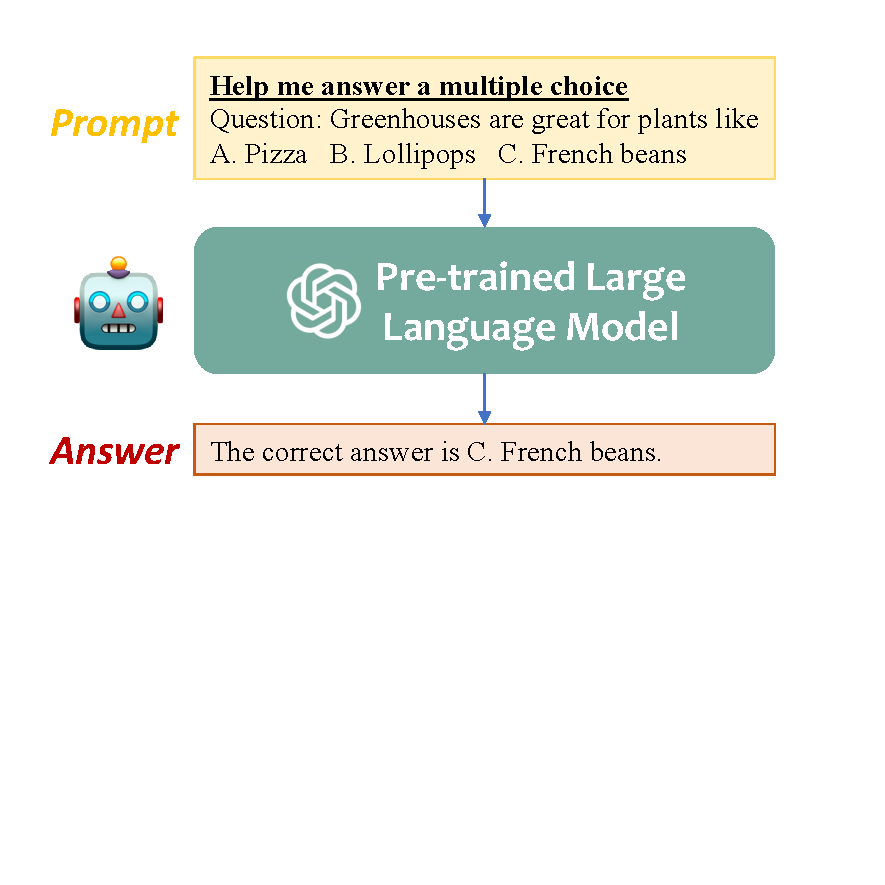
\includegraphics[width=0.45\textwidth]{pic/PromptExample.pdf}
%     \caption{An example of the language prompt. A textual prompt is designed to let the pre-trained large language model perform the multi-choice question-answering task.}
%     \label{fig:PromptExample}
% \end{figure}

\begin{figure}[!t]
\centering
\subfloat[language prompt]{
\label{fig:intro_lang_prompt}
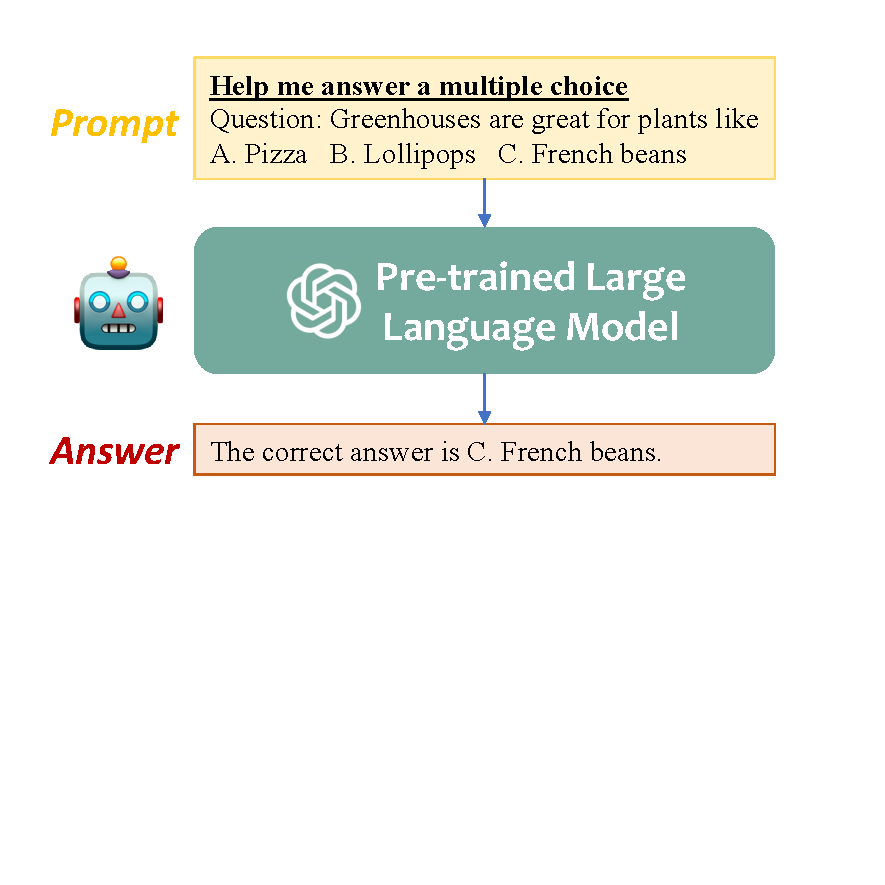
\includegraphics[width=0.36\textwidth]{pic/PromptExample.pdf}%
} \\
\subfloat[graph prompt v.s. graph fine-tune]{
\label{fig:intro_graph_prompt}
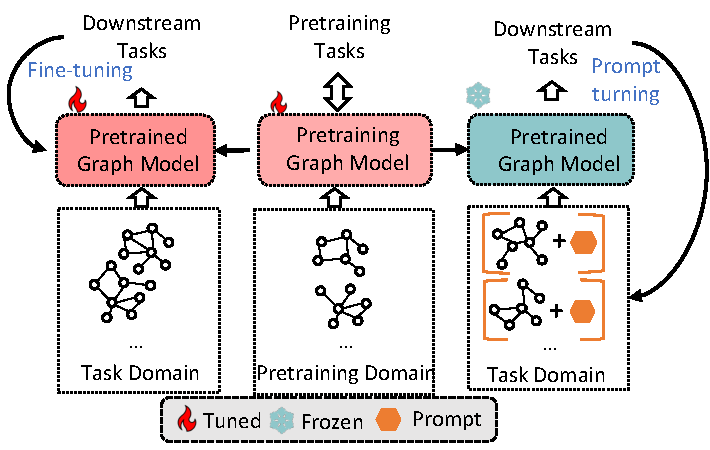
\includegraphics[width=0.44\textwidth]{pic/pt.pdf}%
}
\caption{Language prompt v.s. Graph prompt. A textual prompt is added to the original input to let the pre-trained large language model perform a new task (e.g. the multi-choice question-answering). Inspired by the language prompt, a graph prompt can be also used with graphs in the same way.}\vspace{-3ex}
\label{fig:PromptExample}
\end{figure}


Intuitively, linear structural data like text and images can be perceived as specific instances of a more general non-linear data structure like graphs (a.k.a networks). For instance, a sentence can be treated as a graph path, with words as nodes, and an image can be viewed as a grid graph, where each pixel serves as a graph node. This insight encourages some researchers to explore the transference of successful prompting techniques from existing linear data to the graph area for similar concerns \cite{sun2022gppt, liu2023graphprompt, sun2023all, fang2023universal, zhu2023sglpt, ma2023hetgpt, guo2023datacentric, chen2023ultradp, gong2023prompt}.


However, subsequent studies have found that graph prompts differ substantially from their counterparts in NLP \cite{sun2023all}. \textbf{First}, the design of graph prompts is much more intricate than the formulation of language prompts. Classic language prompts often comprise predefined phrases or learnable vectors appended to input text \cite{brown2020language, gao2021making}. There, the primary focus is on prompt content. In graph learning, however, we do not yet have an equally clear answer to what a graph prompt should look like. A graph prompt involves not only prompt content but also how prompt tokens are structured and integrated into the original graph. \textbf{Second}, aligning downstream graph problems with pre-training tasks is more difficult than in language tasks \cite{liu2023graphprompt, sun2023all}. For example, a typical pre-training approach for a language model is masked word prediction \cite{devlin2019bert}. Many downstream tasks, such as question answering and sentiment classification, can then be reformulated as word-level tasks \cite{liu2023pretrain}. Unlike NLP, where pre-training tasks often share a substantial task sub-space, graph tasks span node-level \cite{grover2016node2vec}, edge-level \cite{zhang2018link}, and graph-level objectives \cite{sun2020infograph, sun2021heterogeneous}, making pre-training pretexts less adaptable. \textbf{Third}, compared with prompts in NLP, which are often understandable phrases, graph prompts are usually less intuitive to non-specialists. Without a more comprehensive analysis, their nature and role within graph models remain somewhat elusive.
% In addition, there are still many unclear questions for us to further understand graph prompting. For example, how effective are these graph prompts? What is their efficiency in terms of parameter complexity and training burden? How powerful and flexible do these prompts manipulate the original graph data?
These questions make it necessary to examine graph prompts more carefully in the context of AGI and to clarify their role in graph learning.




The literature on graph prompting has expanded rapidly in the past few years, but it is still fragmented across different task settings, graph modalities, and adaptation strategies. Existing works often emphasize different perspectives, making direct comparison difficult and slowing the systematic accumulation of knowledge in this area. This survey therefore provides a structured review of how graph prompting addresses the three foundation problems towards AGI discussed above. Beyond that, we further organize the area through the following detailed research questions (RQs):

\begin{itemize}
    \item \textbf{RQ1: How to understand existing work with a unified framework since they are very different?} Our main focus is to understand the various methods used in the field of graph prompting. We want to bring together all these different approaches and ideas to create a single, cohesive framework. This framework will help us thoroughly grasp the existing research and provide a strong foundation for future research in this area.
   \item  \textbf{RQ2: Why Prompt? What's the Nature of Graph Prompt?}
  In this part of our study, we aim to understand why prompts are important. We want to uncover the fundamental aspects of graph prompts. What exactly do graph prompts do in graph problems? How do they fit into the complex graphs, and how do they help us achieve the broader goal of creating AI systems that can handle graph data effectively? These questions highlight the significant role that graph prompts play in shaping the future of AI when dealing with graph information.


   \item  \textbf{RQ3: How to Design Graph Prompts?} Designing good graph prompts is a complex task. In this part, we explore the technical details of designing graph prompts: what do they look like, how do they align downstream tasks and the pre-train task, and how they are learned? These important questions focus on the skill of making prompts that work well with the complexities of graph data, helping researchers make better prompts.





   \item  \textbf{RQ4: How to Deploy Graph Prompts in Real-world Applications?} Easy-to-use toolkits for graph prompting are still limited, and many potential applications remain under-explored. This research question focuses on making graph prompts practical for use in real-world situations with an easily extensible programming package.


   \item  \textbf{RQ5: What Are the Current Challenges and Future Directions in Graph Prompting?} This question guides us to look at the challenges we're dealing with today and the way forward. By tackling these important questions, we hope to provide a roadmap for ongoing graph-prompting research.


\end{itemize}




RQ1 motivates a unified framework for analyzing graph prompt learning. This framework decomposes graph prompts into prompt tokens, token structures, and inserting patterns. Such a higher-level perspective offers a structured understanding of the field and a stable lens for comparing subsequent variants.


RQ2 concerns the relationship between prompts and existing graph models through the lenses of flexibility and expressiveness, leading to a deeper understanding of the nature of graph prompts. Unlike many prompt learning surveys in NLP \cite{liu2023pretrain}, which treat prompting primarily as a mechanism for bridging pre-training and downstream tasks, graph prompting is discussed here as being intertwined with the modeling capacity of graph learners themselves. This perspective helps clarify why prompt learning is promising in the graph domain and how it differs from conventional fine-tuning methods \cite{hu2020strategies}.


RQ3 motivates a comprehensive taxonomy covering over one hundred representative studies through early 2026. The taxonomy organizes these works according to node-level, edge-level, and graph-level settings and aligns them with the broader context of pre-training tasks. This organization clarifies prompt mechanisms within the overall ``pre-training and prompting'' workflow.

RQ4 concerns the supporting ecosystem for graph prompting. ProG (prompt graph) \footnote{\url{https://github.com/sheldonresearch/ProG}} is introduced as a unified Python library, and a companion repository\footnote{\url{https://github.com/WxxShirley/Awesome-Graph-Prompt}} curates graph prompt papers, benchmark datasets, and publicly available implementations. Together, these resources improve accessibility for researchers and practitioners working on graph prompting.

Beyond these questions, the survey further discusses application scenarios, current challenges, and future research directions, thereby outlining a broader roadmap for the development of graph prompt learning (RQ5). The contributions are summarised as follows:

\begin{itemize}
    \item \textbf{Enabling Comprehensive Analysis.} A unified framework is developed for analyzing graph prompt learning, providing a comprehensive view of prompt tokens, token structures, and inserting patterns.
    \item \textbf{Novel Perspectives on Prompt-Model Interplay. } A deeper discussion of the nature of graph prompts is provided. Unlike traditional work that treats prompts mainly as a mechanism for bridging downstream tasks and pre-training objectives, the discussion here examines the flexibility and expressiveness of graph models and develops a more thorough perspective on the interplay between prompts and existing graph learners.
    \item \textbf{A Systematic Taxonomy of Graph Prompting. } The survey synthesizes over one hundred representative studies in graph prompting through early 2026. This taxonomy organizes these contributions and clarifies prompt mechanisms within the overarching ``pre-training and prompting'' workflow.
    % \item \textbf{Quantitative and Qualitative Insights. } We conduct extensive experiments to evaluate different graph prompts and propose a new metric to evaluate how well a graph prompt reformulates graph data.
    \item \textbf{Empowering the Graph Prompting Ecosystem. } ProG, a Python library for graph prompting, and a companion repository of graph prompt research resources are presented.
    \item \textbf{Charting a Path Forward. } A detailed discussion of current challenges and future directions in the field.
\end{itemize}


\textbf{Roadmap.} The remainder of this survey is organized as follows: Section \ref{sec:method} presents the survey methodology, followed by preliminaries in Section \ref{sec:pre}, pre-training methods in Section \ref{sec:pretrain_method}, and prompting methods for graph models in Section \ref{sec:ptask}. Section \ref{sec:app} discusses potential applications of graph prompting, and Section \ref{sec:prog} presents ProG. Section \ref{sec:dis} discusses current challenges and future directions. Section \ref{sec:con} concludes the survey and presents the contribution declaration of the authors.



